\documentclass{standalone}
\usepackage{tikz}
\usetikzlibrary{patterns, positioning}


\begin{document}
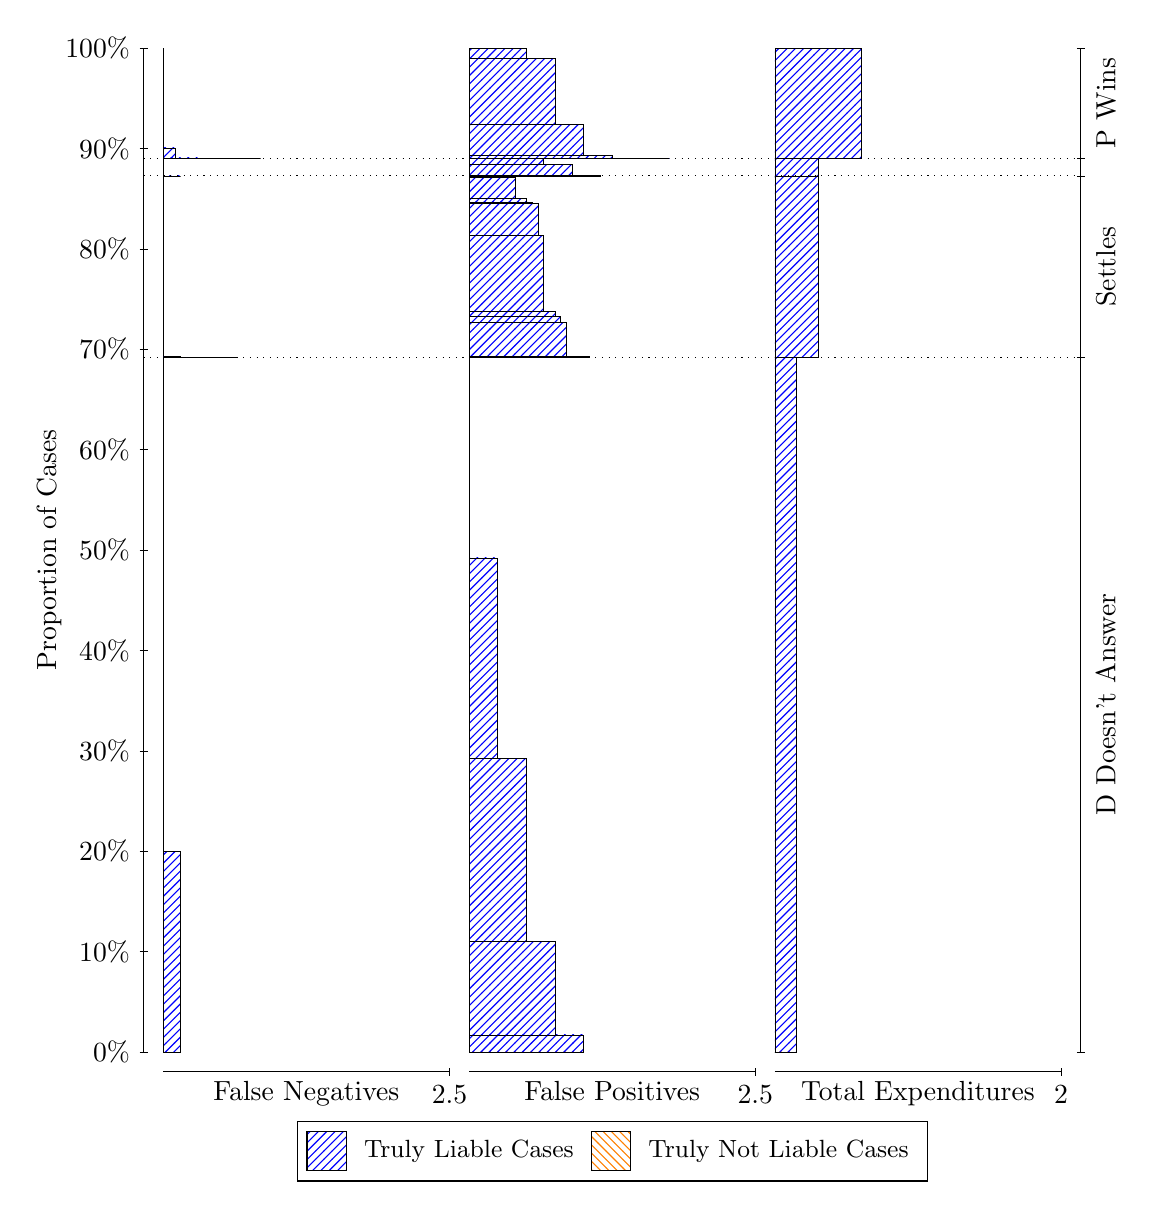
\begin{tikzpicture}
\draw[black, very thin] (1.5,1.75) -- (1.5,14.5);
\node[rotate=90, text=black, anchor=center] at (0.3, 8.125) {Proportion of Cases};
\draw[black, very thin] (1.45,1.75) -- (1.55,1.75);
\node[text=black, anchor=east] at (1.45, 1.75) {0\%};
\draw[black, very thin] (1.45,3.025) -- (1.55,3.025);
\node[text=black, anchor=east] at (1.45, 3.025) {10\%};
\draw[black, very thin] (1.45,4.3) -- (1.55,4.3);
\node[text=black, anchor=east] at (1.45, 4.3) {20\%};
\draw[black, very thin] (1.45,5.575) -- (1.55,5.575);
\node[text=black, anchor=east] at (1.45, 5.575) {30\%};
\draw[black, very thin] (1.45,6.85) -- (1.55,6.85);
\node[text=black, anchor=east] at (1.45, 6.85) {40\%};
\draw[black, very thin] (1.45,8.125) -- (1.55,8.125);
\node[text=black, anchor=east] at (1.45, 8.125) {50\%};
\draw[black, very thin] (1.45,9.4) -- (1.55,9.4);
\node[text=black, anchor=east] at (1.45, 9.4) {60\%};
\draw[black, very thin] (1.45,10.675) -- (1.55,10.675);
\node[text=black, anchor=east] at (1.45, 10.675) {70\%};
\draw[black, very thin] (1.45,11.95) -- (1.55,11.95);
\node[text=black, anchor=east] at (1.45, 11.95) {80\%};
\draw[black, very thin] (1.45,13.225) -- (1.55,13.225);
\node[text=black, anchor=east] at (1.45, 13.225) {90\%};
\draw[black, very thin] (1.45,14.5) -- (1.55,14.5);
\node[text=black, anchor=east] at (1.45, 14.5) {100\%};

\draw[black, very thin] (13.4,1.75) -- (13.4,14.5);
\draw[black, very thin] (13.35,1.75) -- (13.45,1.75);
\node[anchor=west] at (13.35, 1.75) {};
\draw[black, very thin] (13.35,10.575) -- (13.45,10.575);
\node[anchor=west] at (13.35, 10.575) {};
\draw[black, very thin] (13.35,12.877) -- (13.45,12.877);
\node[anchor=west] at (13.35, 12.877) {};
\draw[black, very thin] (13.35,13.102) -- (13.45,13.102);
\node[anchor=west] at (13.35, 13.102) {};
\draw[black, very thin] (13.35,14.5) -- (13.45,14.5);
\node[anchor=west] at (13.35, 14.5) {};

\draw[black, very thin, pattern color=blue, pattern=north east lines] (1.75,1.75) rectangle (1.968,4.2999);
\draw[black, very thin, pattern color=orange, pattern=north west lines] (1.75,4.2999) rectangle (1.75,4.2999);
\draw[black, very thin, pattern color=blue, pattern=north east lines] (1.75,4.2999) rectangle (1.75,10.575);
\draw[black, very thin, pattern color=blue, pattern=north east lines] (1.75,10.575) rectangle (2.6947,10.575);
\draw[black, very thin, pattern color=blue, pattern=north east lines] (1.75,10.575) rectangle (2.5493,10.575);
\draw[black, very thin, pattern color=blue, pattern=north east lines] (1.75,10.575) rectangle (2.404,10.575);
\draw[black, very thin, pattern color=blue, pattern=north east lines] (1.75,10.575) rectangle (2.3313,10.575);
\draw[black, very thin, pattern color=blue, pattern=north east lines] (1.75,10.575) rectangle (2.186,10.575);
\draw[black, very thin, pattern color=blue, pattern=north east lines] (1.75,10.575) rectangle (2.1133,10.575);
\draw[black, very thin, pattern color=blue, pattern=north east lines] (1.75,10.575) rectangle (2.0407,10.575);
\draw[black, very thin, pattern color=blue, pattern=north east lines] (1.75,10.575) rectangle (1.968,10.583);
\draw[black, very thin, pattern color=blue, pattern=north east lines] (1.75,10.583) rectangle (1.8227,10.583);
\draw[black, very thin, pattern color=orange, pattern=north west lines] (1.75,10.583) rectangle (1.75,10.583);
\draw[black, very thin, pattern color=blue, pattern=north east lines] (1.75,10.583) rectangle (1.75,12.877);
\draw[black, very thin, pattern color=blue, pattern=north east lines] (1.75,12.877) rectangle (1.968,12.877);
\draw[black, very thin, pattern color=orange, pattern=north west lines] (1.75,12.877) rectangle (1.75,12.877);
\draw[black, very thin, pattern color=blue, pattern=north east lines] (1.75,12.877) rectangle (1.75,13.102);
\draw[black, very thin, pattern color=blue, pattern=north east lines] (1.75,13.102) rectangle (2.9853,13.102);
\draw[black, very thin, pattern color=blue, pattern=north east lines] (1.75,13.102) rectangle (2.622,13.102);
\draw[black, very thin, pattern color=blue, pattern=north east lines] (1.75,13.102) rectangle (2.2587,13.102);
\draw[black, very thin, pattern color=blue, pattern=north east lines] (1.75,13.102) rectangle (2.2587,13.104);
\draw[black, very thin, pattern color=blue, pattern=north east lines] (1.75,13.104) rectangle (1.8953,13.104);
\draw[black, very thin, pattern color=blue, pattern=north east lines] (1.75,13.104) rectangle (1.8953,13.231);
\draw[black, very thin, pattern color=orange, pattern=north west lines] (1.75,13.231) rectangle (1.75,13.231);
\draw[black, very thin, pattern color=blue, pattern=north east lines] (1.75,13.231) rectangle (1.75,14.5);
\draw[black, very thin, pattern color=orange, pattern=north west lines] (5.6333,1.75) rectangle (7.0867,1.75);
\draw[black, very thin, pattern color=blue, pattern=north east lines] (5.6333,1.75) rectangle (7.0867,1.9673);
\draw[black, very thin, pattern color=blue, pattern=north east lines] (5.6333,1.9673) rectangle (6.7233,3.1518);
\draw[black, very thin, pattern color=blue, pattern=north east lines] (5.6333,3.1518) rectangle (6.36,5.4767);
\draw[black, very thin, pattern color=blue, pattern=north east lines] (5.6333,5.4767) rectangle (5.9967,8.0248);
\draw[black, very thin, pattern color=blue, pattern=north east lines] (5.6333,8.0248) rectangle (5.6333,10.575);
\draw[black, very thin, pattern color=orange, pattern=north west lines] (5.6333,10.575) rectangle (7.1593,10.575);
\draw[black, very thin, pattern color=blue, pattern=north east lines] (5.6333,10.575) rectangle (7.1593,10.579);
\draw[black, very thin, pattern color=orange, pattern=north west lines] (5.6333,10.579) rectangle (6.8687,10.579);
\draw[black, very thin, pattern color=blue, pattern=north east lines] (5.6333,10.579) rectangle (6.8687,11.014);
\draw[black, very thin, pattern color=blue, pattern=north east lines] (5.6333,11.014) rectangle (6.796,11.087);
\draw[black, very thin, pattern color=orange, pattern=north west lines] (5.6333,11.087) rectangle (6.7233,11.087);
\draw[black, very thin, pattern color=blue, pattern=north east lines] (5.6333,11.087) rectangle (6.7233,11.152);
\draw[black, very thin, pattern color=orange, pattern=north west lines] (5.6333,11.152) rectangle (6.578,11.152);
\draw[black, very thin, pattern color=blue, pattern=north east lines] (5.6333,11.152) rectangle (6.578,12.119);
\draw[black, very thin, pattern color=blue, pattern=north east lines] (5.6333,12.119) rectangle (6.5053,12.524);
\draw[black, very thin, pattern color=blue, pattern=north east lines] (5.6333,12.524) rectangle (6.4327,12.545);
\draw[black, very thin, pattern color=blue, pattern=north east lines] (5.6333,12.545) rectangle (6.36,12.59);
\draw[black, very thin, pattern color=blue, pattern=north east lines] (5.6333,12.59) rectangle (6.2147,12.853);
\draw[black, very thin, pattern color=blue, pattern=north east lines] (5.6333,12.853) rectangle (6.142,12.869);
\draw[black, very thin, pattern color=blue, pattern=north east lines] (5.6333,12.869) rectangle (6.0693,12.869);
\draw[black, very thin, pattern color=blue, pattern=north east lines] (5.6333,12.869) rectangle (5.9967,12.869);
\draw[black, very thin, pattern color=blue, pattern=north east lines] (5.6333,12.869) rectangle (5.8513,12.877);
\draw[black, very thin, pattern color=blue, pattern=north east lines] (5.6333,12.877) rectangle (5.7787,12.877);
\draw[black, very thin, pattern color=blue, pattern=north east lines] (5.6333,12.877) rectangle (5.706,12.877);
\draw[black, very thin, pattern color=blue, pattern=north east lines] (5.6333,12.877) rectangle (5.6333,12.877);
\draw[black, very thin, pattern color=orange, pattern=north west lines] (5.6333,12.877) rectangle (7.3047,12.877);
\draw[black, very thin, pattern color=blue, pattern=north east lines] (5.6333,12.877) rectangle (7.3047,12.883);
\draw[black, very thin, pattern color=blue, pattern=north east lines] (5.6333,12.883) rectangle (6.9413,13.019);
\draw[black, very thin, pattern color=blue, pattern=north east lines] (5.6333,13.019) rectangle (6.578,13.101);
\draw[black, very thin, pattern color=blue, pattern=north east lines] (5.6333,13.101) rectangle (6.2147,13.102);
\draw[black, very thin, pattern color=blue, pattern=north east lines] (5.6333,13.102) rectangle (5.8513,13.102);
\draw[black, very thin, pattern color=orange, pattern=north west lines] (5.6333,13.102) rectangle (8.1767,13.102);
\draw[black, very thin, pattern color=blue, pattern=north east lines] (5.6333,13.102) rectangle (8.1767,13.102);
\draw[black, very thin, pattern color=orange, pattern=north west lines] (5.6333,13.102) rectangle (7.8133,13.102);
\draw[black, very thin, pattern color=blue, pattern=north east lines] (5.6333,13.102) rectangle (7.8133,13.103);
\draw[black, very thin, pattern color=orange, pattern=north west lines] (5.6333,13.103) rectangle (7.45,13.103);
\draw[black, very thin, pattern color=blue, pattern=north east lines] (5.6333,13.103) rectangle (7.45,13.14);
\draw[black, very thin, pattern color=orange, pattern=north west lines] (5.6333,13.14) rectangle (7.0867,13.14);
\draw[black, very thin, pattern color=blue, pattern=north east lines] (5.6333,13.14) rectangle (7.0867,13.53);
\draw[black, very thin, pattern color=orange, pattern=north west lines] (5.6333,13.53) rectangle (6.7233,13.53);
\draw[black, very thin, pattern color=blue, pattern=north east lines] (5.6333,13.53) rectangle (6.7233,14.371);
\draw[black, very thin, pattern color=blue, pattern=north east lines] (5.6333,14.371) rectangle (6.36,14.498);
\draw[black, very thin, pattern color=blue, pattern=north east lines] (5.6333,14.498) rectangle (5.9967,14.5);
\draw[black, very thin, pattern color=blue, pattern=north east lines] (5.6333,14.5) rectangle (5.6333,14.5);
\draw[black, very thin, pattern color=orange, pattern=north west lines] (9.5167,1.75) rectangle (9.7892,1.75);
\draw[black, very thin, pattern color=blue, pattern=north east lines] (9.5167,1.75) rectangle (9.7892,10.575);
\draw[black, very thin, pattern color=orange, pattern=north west lines] (9.5167,10.575) rectangle (10.062,10.575);
\draw[black, very thin, pattern color=blue, pattern=north east lines] (9.5167,10.575) rectangle (10.062,12.877);
\draw[black, very thin, pattern color=orange, pattern=north west lines] (9.5167,12.877) rectangle (10.062,12.877);
\draw[black, very thin, pattern color=blue, pattern=north east lines] (9.5167,12.877) rectangle (10.062,13.102);
\draw[black, very thin, pattern color=orange, pattern=north west lines] (9.5167,13.102) rectangle (10.607,13.102);
\draw[black, very thin, pattern color=blue, pattern=north east lines] (9.5167,13.102) rectangle (10.607,14.5);
\draw[black, dotted] (1.5,10.575) -- (13.4,10.575);
\draw[black, dotted] (1.5,12.877) -- (13.4,12.877);
\draw[black, dotted] (1.5,13.102) -- (13.4,13.102);
\draw[black, very thin] (1.75,1.5) -- (5.3833,1.5);
\node[text=black, anchor=north] at (3.5667, 1.5) {False Negatives};
\draw[black, very thin] (5.3833,1.45) -- (5.3833,1.55);
\node[text=black, anchor=north] at (5.3833, 1.45) {2.5};

\draw[black, very thin] (5.6333,1.5) -- (9.2667,1.5);
\node[text=black, anchor=north] at (7.45, 1.5) {False Positives};
\draw[black, very thin] (9.2667,1.45) -- (9.2667,1.55);
\node[text=black, anchor=north] at (9.2667, 1.45) {2.5};

\draw[black, very thin] (9.5167,1.5) -- (13.15,1.5);
\node[text=black, anchor=north] at (11.333, 1.5) {Total Expenditures};
\draw[black, very thin] (13.15,1.45) -- (13.15,1.55);
\node[text=black, anchor=north] at (13.15, 1.45) {2};

\node[text=black, centered, rotate=90] at (13.72, 6.1623) {D Doesn't Answer};
\node[text=black, centered, rotate=90] at (13.72, 11.726) {Settles};

\node[text=black, centered, rotate=90] at (13.72, 13.801) {P Wins};

\draw (7.449999999999999,1.5) node[draw=none] (baseCoordinate) {};
\begin{scope}[align=center]
        \matrix[scale=0.5, draw=black, below=0.5cm of baseCoordinate, nodes={draw}, column sep=0.1cm]{
            \node[rectangle, draw, minimum width=0.5cm, minimum height=0.5cm, pattern color=blue, pattern=north east lines] {}; &
            \node[draw=none, font=\small, text=black] (B) {Truly Liable Cases}; &
            \node[rectangle, draw, minimum width=0.5cm, minimum height=0.5cm, pattern color=orange, pattern=north west lines] {}; &
            \node[draw=none, font=\small, text=black] (B) {Truly Not Liable Cases}; \\
            };
\end{scope}

\end{tikzpicture}
\end{document}